\documentclass[12pt]{article}
\setlength{\parskip}{0.2cm}
\setlength{\parindent}{0.5cm}
 
\usepackage[margin=1in]{geometry} 
\usepackage{amsmath,amsthm,amssymb}
\usepackage{graphicx}
\usepackage[english]{babel}
\usepackage{hyperref}
\usepackage{subcaption}

\begin{document}


\title{Homework 4 - Report}
\author{Álvaro Martínez Alfaro\\
    Autonomous Robotics}

\maketitle

\section{Introduction}

This report presents the development and evaluation of a reactive navigation system for a simulated
mobile robot in the \textbf{Flatland} environment under \textbf{ROS2}. Flatland is a lightweight 2D
simulatoir that enables rapid prototyping of robotic algorithms without the overhead of 3D physics
engines.

The scenario consists of a robot equipped with a 360° LiDAR sensor navigating a $10 \times 6$m
bounded arena in which four goal objects are placed at fixed positions. The robot's baseline
behavior follows a simple reactive loop: move forward until an obstacle is detected, then turn in a
random direction. This work extends the baseline through four progressive steps: (i) implementing a
\textbf{goal detector} that uses laser readings to identify and remove goals upon close proximity,
(ii) an \textbf{improved navigation} strategy that selects the direction with the most free space
instead of turning randomly, (iii) systematic \textbf{experimentation} across different navigation
modes, linear speeds, and laser ranges, and (iv) the design and evaluation of \textbf{custom maps}
to assess the robustness of the developed behaviors.

The remainder of the report is structured as follows: Section \ref{sec:implementation} details the
implementation of each component, Section \ref{sec:experimentation} presents the experimental
results, and Section \ref{sec:conclusion} draws conclusions from the work.

%------------------------------------------------

\section{Implementation details} \label{sec:implementation}

The entire implementation is contained in two files: \texttt{\_\_init\_\_.py}, which defines the
\textbf{Controller} ROS2 node responsible for robot perception, navigation, goal detection and
experiment management; and \texttt{homework4.launch.py}, which exposes configurable arguments for
the map type and output \texttt{csv} file.

\subsection{Goal detector}

Goal detection runs on every laser callback via \texttt{process\_obstacle\_detection}, which
iterates over all remaining active obstacles and calls \texttt{should\_remove\_obstacle} for each
one. This function applies a two-condition check:

\begin{enumerate}
    \item \textbf{Proximity filter}: computes the Euclidean distance from the robot pose to the
          obstacle's known position. If it exceeds the \texttt{obstacle\_detection\_distance}
          threshold (1.0 m), the check is skipped immediately.
    \item \textbf{Laser confirmation}: converts the vector to the obstacle into a robot-relative
          angle (\texttt{global\_angle - robot\_theta}, normalized to $[-\pi, \pi]$), maps the angle
          to a laser scan index via \texttt{angle\_to\_scan\_index}, then reads the average laser
          range at that index using \texttt{get\_mean\_range} (a windowed average over $\pm$
          \texttt{mean\_window}) neighboring rays). If the difference between the laser reading and
          the computed distance is within the \texttt{obstacle\_match\_tolerance} (0.2 m), the
          obstacle is confirmed and removed from the active list.
\end{enumerate}

When a goal is confirmed, \texttt{remove\_obstacle} relocates it off-map via Flatland's
\texttt{MoveModel} service, records the elapsed time since run start (for experimentation purposes),
and removes it from the active set. When the last obstacle is removed, the run ends.

Here, the key parameters are the \texttt{obstacle\_detection\_distance}, which limits the search to
a radius around the robot and is set to $1.0$m; the \texttt{obstacle\_match\_tolerance},
which accounts for sensor noise and map inaccuracies and is set to $0.2$m; and the
\texttt{mean\_window}, which smooths laser readings to improve robustness and its values vary per
experiment ($2$ or $4$).

\subsection{Improved navigation}

The navigation decision is made inside \texttt{lidar\_callback}. On each scan, the averaged front
laser reading (index $\lfloor N/2 \rfloor$, window = \texttt{mean\_window}) is compared against
\texttt{min\_distance} ($0.8$m). If the path ahead is blocked, the controller triggers a rotation,
either random or heuristic depending on the current \texttt{nav\_mode}.

In the \textbf{random} mode (\texttt{start\_random\_rotation}), the robot simply picks a random
angular speed uniformly in $[-\pi, \pi]$ rad/s. In the \textbf{improved} mode
(\texttt{start\_heuristic\_rotation}), the robot scans all $N$ laser rays and finds the index with
the highest windowed average range (window = \texttt{mean\_window}). It derives the corresponding
robot-relative angle and turns at $\pm 1.5$ rad/s, positive (left) if the angle is $\ge 0$ and
negative (right) otherwise.

In both modes, \texttt{rotation\_iterations\_left} is set to \texttt{random\_rotation\_iterations}
(10) and counted down each callback tick, during which the robot rotates in place.

Additionally, a stuck detection mechanism was added to handle cases where the robot might get
trapped in a corner or against a wall. Every 5 seconds, the controller checks whether the robot has
moved at least $0.4$ m. If not, it triggers a two-phase escape: first, it reverses for 20 callback
ticks, and then it performs a random spin for 35 ticks before resuming normal navigation.

Finally, the key parameters here are the \texttt{min\_distance} threshold for obstacle avoidance,
which is set to $0.8$m; the \texttt{random\_rotation\_iterations}, which determines how long the
robot rotates, set to $10$ iterations; and the turn speed fixed at $1.5$ rad/s in the improved mode.

\subsection{Map generation}

Maps in Flatland are defined by grayscale \textit{PNG} images paired with a \textit{YAML}
configuration file. Black pixels (0) are treated as walls, while white pixels (255) represent free
space. The \textit{YAML} sets the map resolution ($0.05$ m/pixel) and the origin ($-5.0, -3.0$), so
the $200 \times 120$ pixel image maps to a $10 \times 6$ m world with $(0,0)$ at the center.

The script \texttt{image\_generator.py} uses the \textit{PIL} library to programmatically draw three
maps:

\begin{itemize}
    \item \textbf{Rectangular map}: only the four outer walls are present, creating a simple open
          arena for baseline testing.
    \item \textbf{Line map}: adds a thin vertical wall near the center ($6$ pixels wide $\times$
          $40$ pixels tall $= 0.3 \times 2.0$ m). It creates a partial barrier that splits the arena
          symmetrically.
    \item \textbf{TP map}: two offset rectangular pillars placed diagonally across the arena.
\end{itemize}

The three maps are shown in Figure \ref{fig:maps}. Both custom maps are designed to avoid the four
goal positions ($\pm 2.5, \pm 1.5$), so goals remain reachable in all configurations. Each map has
its own \texttt{world\_*.yaml} and \texttt{*\_map.yaml} and can be selected at launch via the
\texttt{world\_name} argument.

\begin{figure}
    \centering
    \begin{subfigure}[b]{0.32\textwidth}
        
\includegraphics[width=\textwidth]{figures/rect_map.png}
        \caption{Rect map (baseline)}
    \end{subfigure}
    \hfill
    \begin{subfigure}[b]{0.32\textwidth}
        
\includegraphics[width=\textwidth]{figures/line_map.png}
        \caption{Line map}
    \end{subfigure}
    \hfill
    \begin{subfigure}[b]{0.32\textwidth}
        
\includegraphics[width=\textwidth]{figures/tp_map.png}
        \caption{TP map}
    \end{subfigure}
    \caption{The three maps used in the experiments.}
    \label{fig:maps}
\end{figure}

%------------------------------------------------

\section{Experimentation} \label{sec:experimentation}

The experiments were conducted across \textbf{12 configurations}, combining 2 navigation modes
(basic and improved), 3 linear speeds ($0.5$, $1.0$ and $2.0$ m/s), and 2 laser window sizes ($2$
and $4$), each repeated \textbf{10 times per map}. The same set of configurations was tested on
three maps: the baseline rect map, and the two custom maps (line and tp). The metric recorded is the
total time to detect and remove all four goals, defined as the elapsed time from run start to the
last goal removal. Between runs, the robot and all goals are automatically reset to their initial
positions. The results are summarized in Tables \ref{tab:rect_map}, \ref{tab:line_map} and
\ref{tab:x_map}.

\begin{table}
    \centering
    \begin{tabular}{llcc}
        \hline
        \textbf{Nav mode} & \textbf{Speed (m/s)} & \textbf{Window} & \textbf{Mean time (s)} \\
        \hline
        Basic             & 0.5                  & 2               & 80.71                  \\
                          & 0.5                  & 4               & 186.86                 \\
                          & 1.0                  & 2               & 34.70                  \\
                          & 1.0                  & 4               & 84.59                  \\
                          & 2.0                  & 2               & 12.39                  \\
                          & 2.0                  & 4               & 12.39                  \\
        Improved          & 0.5                  & 2               & 81.93                  \\
                          & 0.5                  & 4               & 191.63                 \\
                          & 1.0                  & 2               & 32.98                  \\
                          & 1.0                  & 4               & 78.14                  \\
                          & 2.0                  & 2               & 12.39                  \\
                          & 2.0                  & 4               & 12.39                  \\
        \hline
    \end{tabular}
    \caption{Mean completion time per configuration --- Rect Map.}
    \label{tab:rect_map}
\end{table}

\begin{table}
    \centering
    \begin{tabular}{llcc}
        \hline
        \textbf{Nav mode} & \textbf{Speed (m/s)} & \textbf{Window} & \textbf{Mean time (s)} \\
        \hline
        Basic             & 0.5                  & 2               & 153.05                 \\
                          & 0.5                  & 4               & 171.41                 \\
                          & 1.0                  & 2               & 47.34                  \\
                          & 1.0                  & 4               & 67.09                  \\
                          & 2.0                  & 2               & 12.39                  \\
                          & 2.0                  & 4               & 12.49                  \\
        Improved          & 0.5                  & 2               & 151.85                 \\
                          & 0.5                  & 4               & 197.49                 \\
                          & 1.0                  & 2               & 62.48                  \\
                          & 1.0                  & 4               & 73.88                  \\
                          & 2.0                  & 2               & 12.39                  \\
                          & 2.0                  & 4               & 12.49                  \\
        \hline
    \end{tabular}
    \caption{Mean completion time per configuration --- Line Map.}
    \label{tab:line_map}
\end{table}

\begin{table}
    \centering
    \begin{tabular}{llcc}
        \hline
        \textbf{Nav mode} & \textbf{Speed (m/s)} & \textbf{Window} & \textbf{Mean time (s)} \\
        \hline
        Basic             & 0.5                  & 2               & 146.41                 \\
                          & 0.5                  & 4               & 297.42                 \\
                          & 1.0                  & 2               & 117.15                 \\
                          & 1.0                  & 4               & 165.63                 \\
                          & 2.0                  & 2               & 85.30                  \\
                          & 2.0                  & 4               & 72.76                  \\
        Improved          & 0.5                  & 2               & 121.57                 \\
                          & 0.5                  & 4               & 190.09                 \\
                          & 1.0                  & 2               & 70.72                  \\
                          & 1.0                  & 4               & 106.45                 \\
                          & 2.0                  & 2               & 45.54                  \\
                          & 2.0                  & 4               & 54.29                  \\
        \hline
    \end{tabular}
    \caption{Mean completion time per configuration --- TP Map.}
    \label{tab:x_map}
\end{table}



\subsection{Effect of linear speed}

Linear speed is by far the dominant factor across all configurations and maps. At $2.0$ m/s the
robot detects all goals in less than $100$ seconds consistently, while at $0.5$ m/s it takes between
$80$ and $250$ seconds, depending on the map. The boxplot in Figure \ref{fig:boxplot} confirms that
variance at $2.0$ m/s is essentially zero or very low, which might be due to the fact that the robot
follows the same deterministic path every run, while at $0.5$ m/s it is very high, especially on the
tp map, maybe because the robot has to do more obstacle avoidance maneuvers, following different
paths each time. At $1.0$ m/s results are intermediate but with notable variance depending on the
window size, as discussed in Section \ref{sec:window}.

\begin{figure}
    \centering
    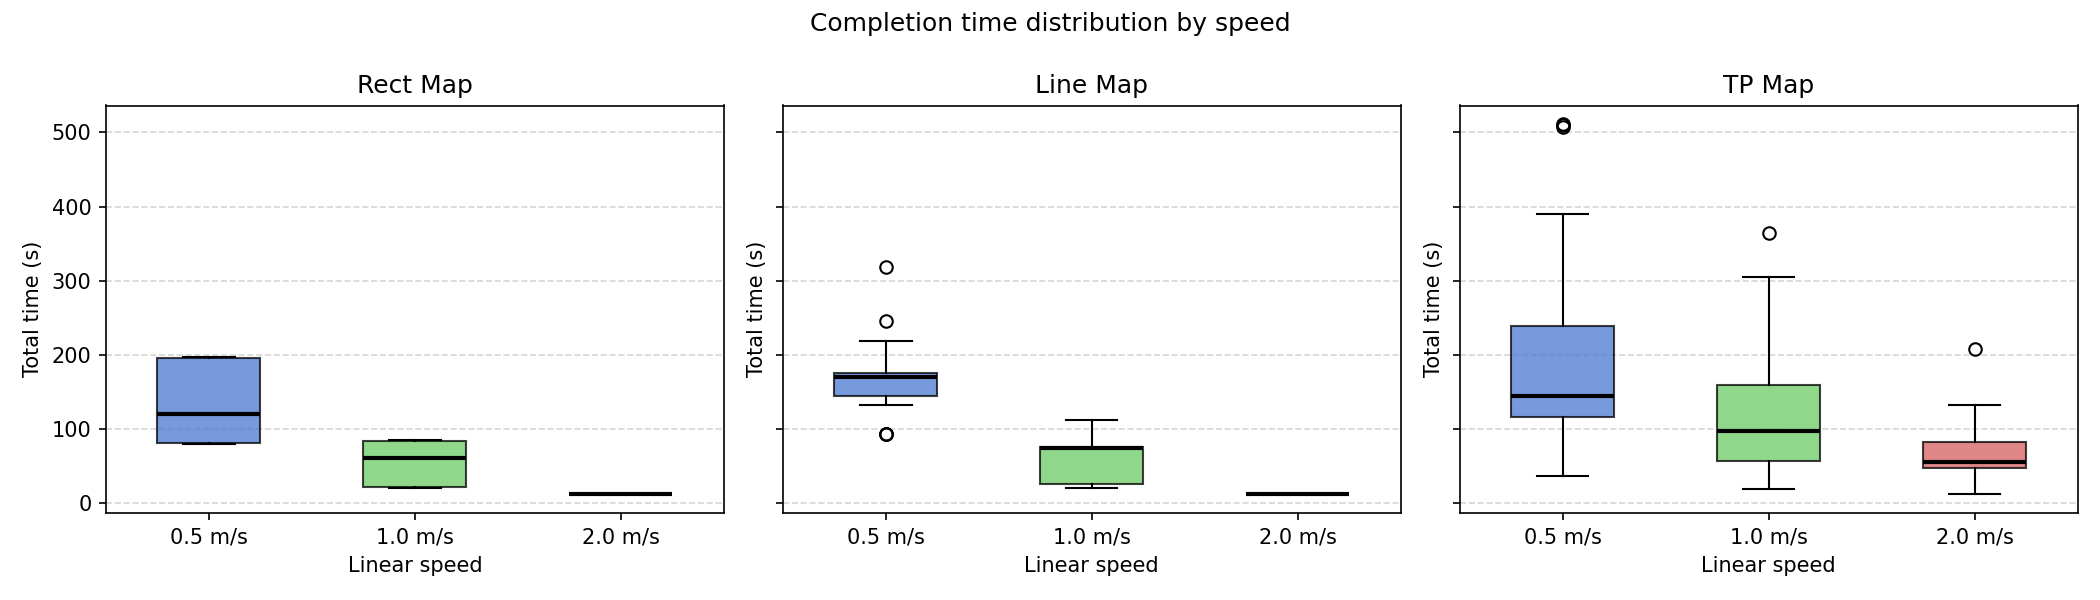
\includegraphics[width=\textwidth]{figures/plot_boxplot_speed.png}
    \caption{Completion time distribution by linear speed across the three maps.}
    \label{fig:boxplot}
\end{figure}

\subsection{Effect of navigation mode}

The improved navigation mode, which selects the direction with the most free space instead of
turning randomly, shows surprisignly \textbf{little improvement} over the basic mode. As shown in
Figure \ref{fig:navmode}, at $2.0$ m/s both modes produce identical results across all maps; the
robot is fast enough to reach all goals via the same deterministic path regardless of how it turns.
At lower speeds, the differences are small and inconsistent; in some configurations the improved
mode is marginally better, while in others the random mode performs equally well or even slightly
better. This suggests that in relatively simple environments, like an open arena with few obstacles,
most directions offer \textit{similar free space} when an obstacle is encountered, giving the
heuristic \textit{little to exploit} over a random choice.

\begin{figure}
    \centering
    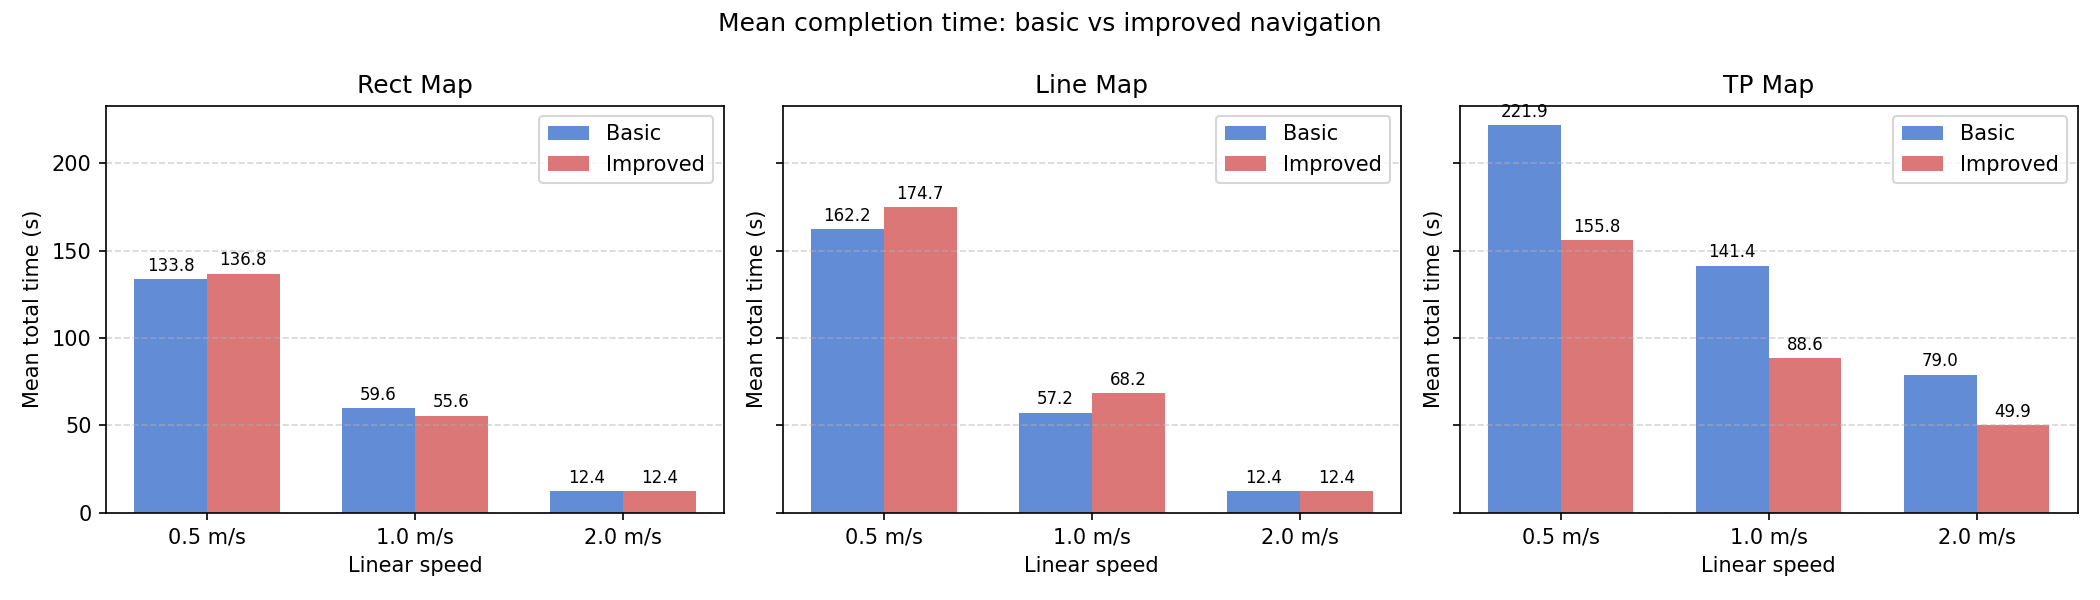
\includegraphics[width=\textwidth]{figures/plot_nav_mode_vs_speed.png}
    \caption{Mean completion time: basic vs improved navigation mode.}
    \label{fig:navmode}
\end{figure}

\subsection{Effect of laser window size} \label{sec:window}

The laser window size has a more notable effect than the navigation mode, particularly at $1.0$ m/s.
As shown in Figure \ref{fig:window}, with $\text{window}=4$ at $1.0$ m/s the robot takes around $84$
seconds consistently across all 10 runs on the rect map, with essentially zero variance. With
$\text{window}=2$ at the same speed, completion times drop to a $20$--$60$ second range with much
higher variance. This is a counterintuitive result, as one would expect that a larger averaging
window should reduce sensor noise, leading to more reliable obstacle detection and better navigation
decisions. Instead, it causes the robot to follow a path that happens to be suboptimal. At $2.0$ m/s
the window has no effect since the robot is fast enough to always follow the same path, while at
$0.5$ m/s both windows produce similarly high and variable completion times.

\begin{figure}
    \centering
    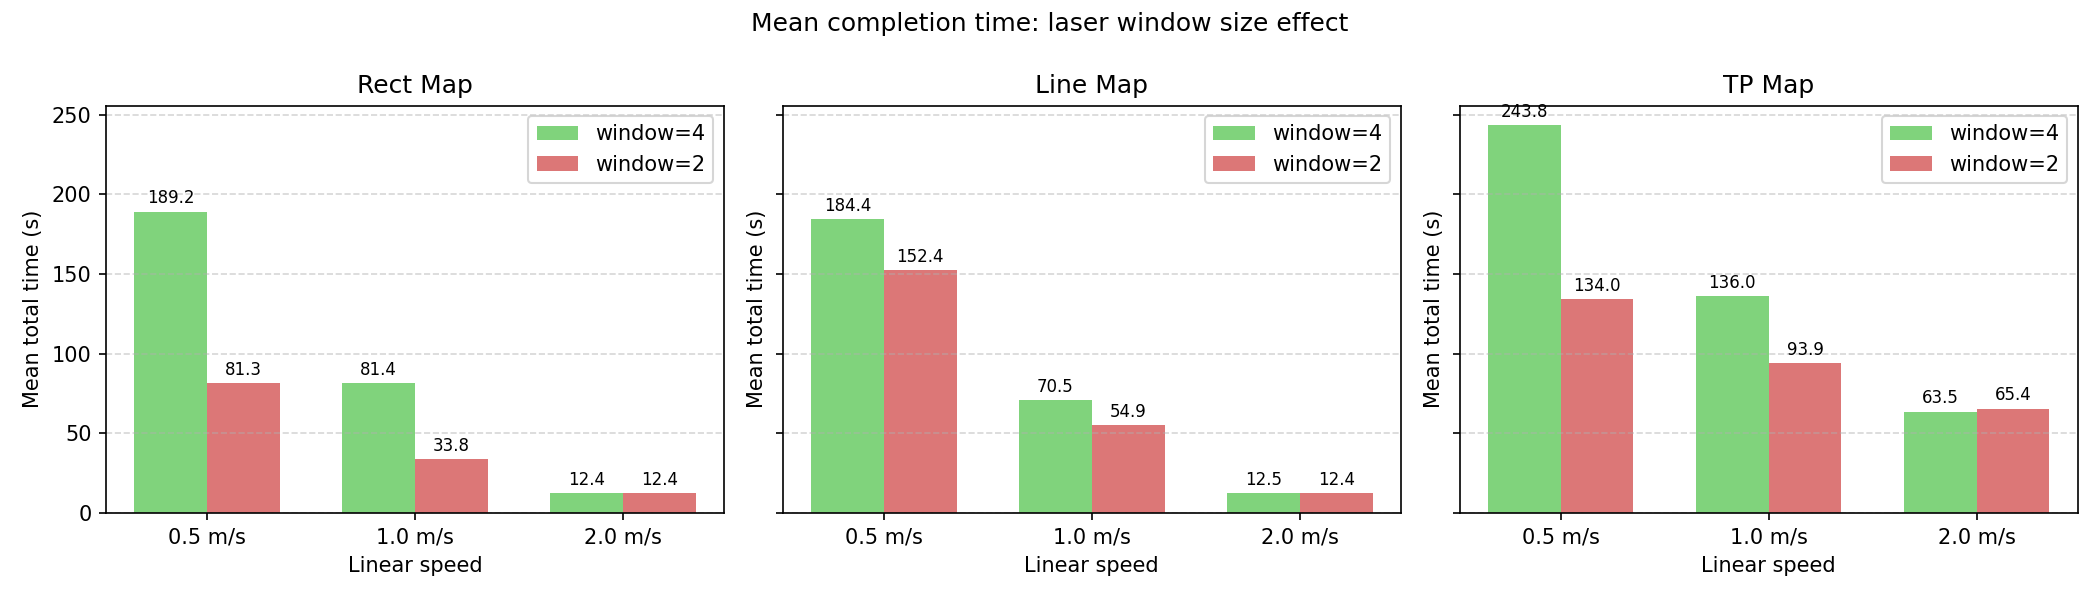
\includegraphics[width=\textwidth]{figures/plot_window_vs_speed.png}
    \caption{Mean completion time: effect of laser window size.}
    \label{fig:window}
\end{figure}

\subsection{Map comparison}

At $2.0$ m/s the rect and line maps show identical completion times, while the tp map is slightly
higher, reaching around a minute on average. This is expected since the tp map has two obstacles
that may force the robot to change its path more often, while the line map has only one thin wall
that can be easily circumvented. At lower speeds, the maps diverge more significantly. The line and
tp maps introduce additional variance compared to the rect map, as the robot must navigate around
the internal obstacles, following different paths each run. The tp map is the hardest at $0.5$ m/s,
producing the highest and most variable completion times across all configurations.

Overall, the map complexity has a secondary effect compared to linear speed, but it amplifies the
variance already observed at lower speeds. Figure \ref{fig:mapcomp} summarises the mean completion
time per map and speed.

\begin{figure}
    \centering
    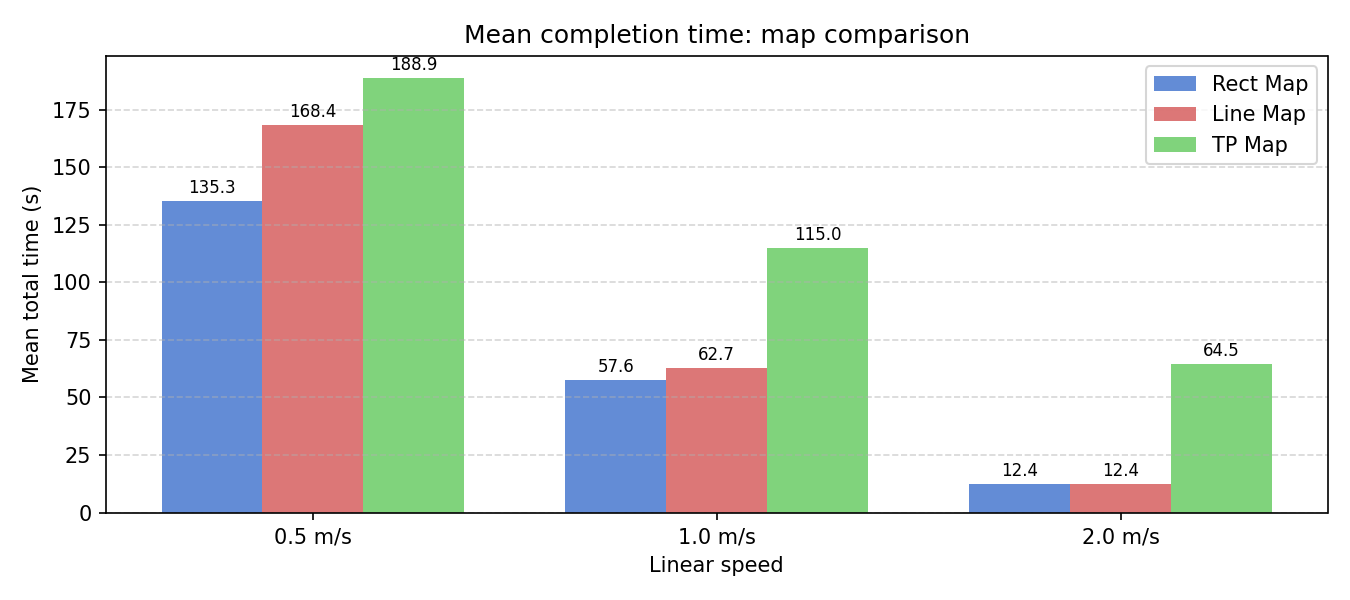
\includegraphics[width=0.75\textwidth]{figures/plot_map_comparison.png}
    \caption{Mean completion time across maps by linear speed.}
    \label{fig:mapcomp}
\end{figure}

%------------------------------------------------

\section{Conclusion} \label{sec:conclusion}

This report presented the development and evaluation of a reactive navigation system for a simulated
mobile robot in the Flatland environment under ROS2. The system was built incrementally, starting
froim a baseline random-turn controller, a laser-based goal detector was added, the navigation
strategy was improved with a free-space heuristic, and the whole system was tested across multiple
configurations and three maps of increasing complexity.

The experiments revealed that linear speed is the dominant factor in performance, with the robot
completing all goals in less than a minute at $2.0$ m/s regardless of the map or navigation mode.
The improved navigation mode showed little to no advantage over the basic one, which can be
attributed to the relative openness of the arenas tested, where most directions offer similar free
space when an obstacle is encountered, leaving the heuristic little to exploit. A more unexpected
finding was the deterministic loop caused by the larger laser window size at $1.0$ m/s, where the
robot consistently followed the same suboptimal path, while the smaller window introduced enough
variability to allow for faster completion times in some runs. The tp map proved to be the most
challenging scenario, particularly for the basic mode at low speeds.

As a final remark, there is one aspect that could be further explored or improved with additional
time, that is testing on more complex maps, such as narrow corridors or maze-like layouts,
would create situations where the free-space heuristic has a real advantage over random turning,
allowing a fairer comparison between the two navigation modes.

\end{document}
